%\documentclass[english, times, mirror]{revdetua}
% use this if you're writing in portuguese:
\documentclass[portuguese, times, mirror]{revdetua}

\usepackage[utf8]{inputenc}
\usepackage{graphicx}
\usepackage{hyperref}

\usepackage{amsmath}
\usepackage{mathtools}

\usepackage{caption}
\usepackage{listings}
\usepackage{color}

\definecolor{dkgreen}{rgb}{0,0.6,0}
\definecolor{gray}{rgb}{0.5,0.5,0.5}
\definecolor{mauve}{rgb}{0.58,0,0.82}

\lstset{frame=tb,
  language=Java,    
  aboveskip=3mm,
  belowskip=3mm,
  showstringspaces=false,
  columns=flexible,
  basicstyle={\small\ttfamily},
  numbers=none,
  numberstyle=\tiny\color{gray},
  keywordstyle=\color{blue},
  commentstyle=\color{dkgreen},
  stringstyle=\color{mauve},
  breaklines=true,
  breakatwhitespace=true,
  tabsize=3
}

\usepackage{tikz}
\usepackage{pgfplots}

% correct bad hyphenation here
\hyphenation{op-tical net-works semi-conduc-tor}

\begin{document}

\Header{1}{5}{Outubro}{2016}{1}
% Note: the month must be in Portuguese

\title{Visão por Computador 2016-17, Guia Prático N.º 10}
\author{Rui Oliveira, Tomás Rodrigues\\ DETI, Universidade de Aveiro \\ Aveiro, Portugal \\ \{ruipedrooliveira, tomasrodrigues\}@ua.pt}
% you should be able to use the \and keyword, but the deti format doesn't like it, for some reason
\maketitle

\begin{resumo}


Pretende-se através deste relatório expor sob forma escrita, o nosso desempenho e objetivos alcançados na aula prática n.º10 da unidade curricular de Visão por Computador do Mestrado Integrado de Engenharia de Computadores e Telemática.

Neste relatório pretenderemos explicar as soluções por nós encontradas para a resolução dos diferentes problemas propostos.


\end{resumo} 

\begin{palavraschave} %
visão, computador, imagem digital, template matching, face detector opencv, c++, 
 \end{palavraschave} %


\section{Repositório: código fonte}


Todas as soluções dos problemas propostos estão disponível através do seguinte repositório (gitHub) criado para o efeito. \\

\href{http://github.com/toomyy94/CV1617-68779-68129}{http://github.com/toomyy94/CV1617-68779-68129}
\\


A resolução dos problemas do presente guia encontram-se na pasta aula10. Para a resolução dos exercícios foi utilizado o CodeBlocks IDE. . 



\section{Problemas propostos}

\subsection{Problema \#1 }

\subsubsection{Enunciado}
\textit{Develop a program to perform traffic sign detection. You can consider the existence of a database with images of several traffic signs (templates) and your program has to find the position of the signs in the input image (or video) if they appear there.
As starting point, explore the OpenCv tutorial about template matching. In your implementation, explore the several matching methods available in OpenCV.}


\subsubsection{Resolução do problema}

No geral pensamos ter conseguido bons resultados na resolução do problema proposto(identificação de um sinal de trânsito em imagens).

Para a resolução deste problema numa 1ª fase criamos a matriz resultante da imagem a procurar e da imagem \textit{template}:

\begin{lstlisting}[caption=Create the result matrix,label=code:C]
int result_cols =  img.cols - templ.cols + 1;
int result_rows = img.rows - templ.rows + 1;

result.create( result_rows, result_cols, CV_32FC1 );
\end{lstlisting}

Depois disso vai-se fazendo deslizar a imagem template na original calculando possíveis matchs ou probabilidades de match:

\begin{lstlisting}[caption=Matching and Normalize,label=code:C]
  matchTemplate( img, templ, result, match_method );
  normalize( result, result, 0, 1, NORM_MINMAX, -1, Mat() );
\end{lstlisting}

São usados 5 algoritmos para o \textit{SQDIFF} e o \textit{SQDIFF\_NORMED}, os melhores casos são os valores calculados correspondentes aos mais baixos, para os outros algoritmos os melhores valores, são os valores mais altos.

\begin{lstlisting}[caption=Desenho de retangulos no ponto de interesse,label=code:C]
if( match_method  == CV_TM_SQDIFF || match_method == CV_TM_SQDIFF_NORMED )
    { matchLoc = minLoc; }
  else
    { matchLoc = maxLoc; }

  rectangle( img_display, matchLoc, Point( matchLoc.x + templ.cols , matchLoc.y + templ.rows ), Scalar::all(0), 2, 8, 0 );
  rectangle( result, matchLoc, Point( matchLoc.x + templ.cols , matchLoc.y + templ.rows ), Scalar::all(0), 2, 8, 0 );
\end{lstlisting}

No código acima vemos o desenho de um retângulo centrado no ponto de interesse calculado como "melhor" na imagem a procurar, o outro retângulo é desenhado numa imagem adicional criado pelo algoritmo de processamento centrada no mesmo local.

\subsubsection{Resultados e principais conclusões}

Nos seguintes testes foi utilizada como template a procurar a seguinte imagem:

\begin{figure}[ht!]
\centering

\includegraphics[width=40mm]{img/stop.jpg}
\caption{Imagem template}
\end{figure}

Num primeiro teste foi utilizada uma imagem padrão com vários sinais de trânsito,  da qual a imagem template foi tirada, por isso esperávamos bons resultados que foram atingidos, sendo a imagem encontrada facilmente no sítio correto.

\begin{figure}[ht!]
\centering
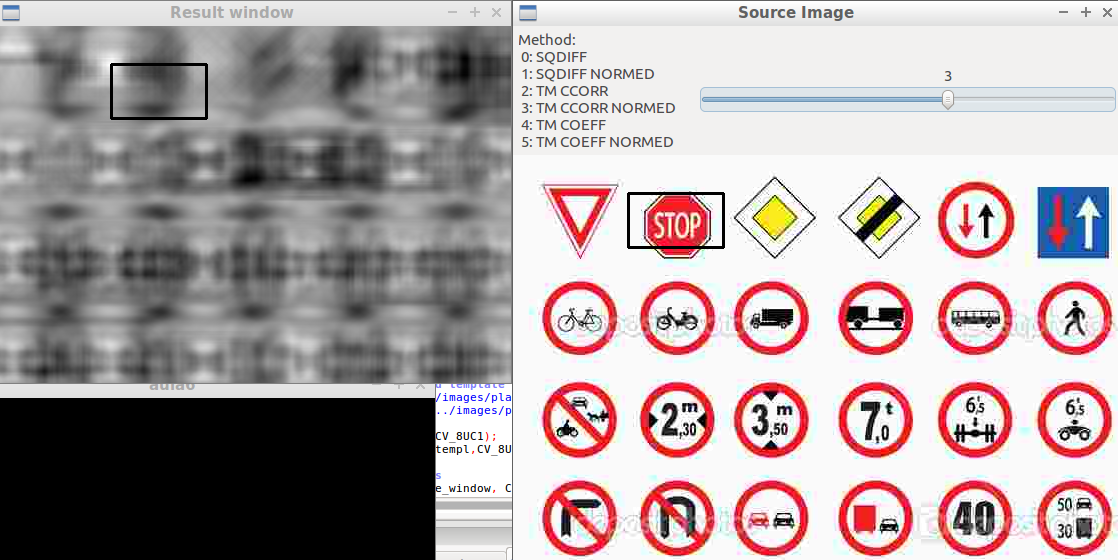
\includegraphics[width=70mm]{img/ex1_1.png}
\caption{Resultado obtido após exercício 1}
\end{figure}

\newpage

Após este teste decidimos ir buscar uma imagem de um ambiente mais real e com vários sinais de "STOP" para ver como o programa reagiria. Os resultados encontrados foram também bons e interessantes, no sentido de que, nuns algoritmos a imagem template foi encontrada no sinal do meio(Figura 3), e com o algoritmo \textit{TM COEFF NORMED(5)} foi encontrado o melhor ponto de "match" no sinal da esquerda(Figura 4) como podemos ver nas imagens abaixo:

\begin{figure}[ht!]
\centering
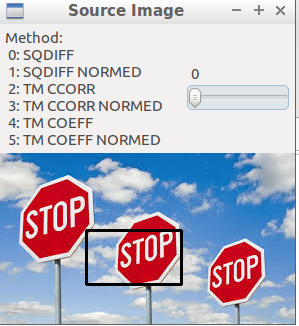
\includegraphics[width=70mm]{img/ex1_2.png}
\caption{Resultado obtido após imagem 2}
\end{figure}

\begin{figure}[ht!]
\centering
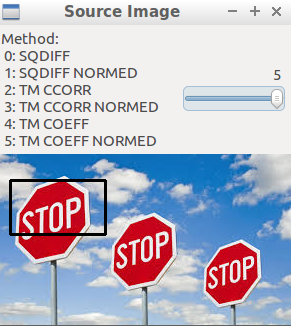
\includegraphics[width=70mm]{img/ex1_3.png}
\caption{Resultado obtido após imagem 2 com outro algoritmo}
\end{figure}

\newpage

Após estes testes ficamos intrigados e fomos ainda fazer um último teste rodando a imagem inicial 90º para a esquerda para ver como o template match reagiria, sendo a imagem inicial bem encontrada em 4 dos 5 algoritmos utilizados.

\begin{figure}[ht!]
\centering
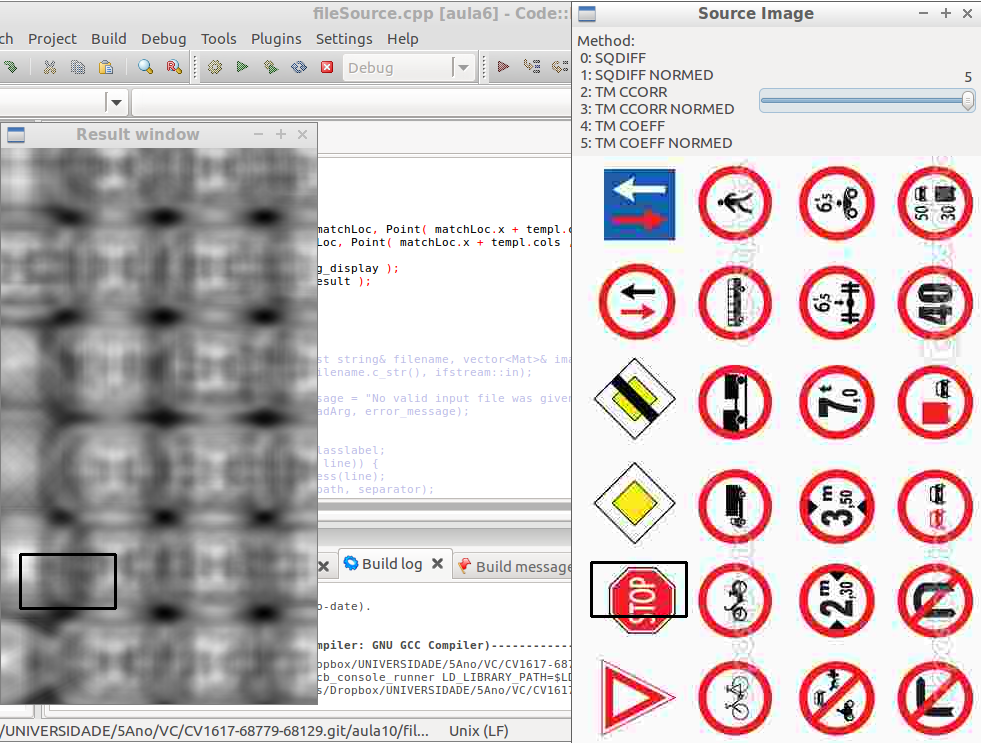
\includegraphics[width=70mm]{img/ex1_4.png}
\caption{Resultado obtido após virar a Figura 1 90º}
\end{figure}

%%%%%%%%%%%%%%%%%%%%%%%%%%%%%%%%%%%%%%%%%%%%%%%%%%%%%%%%%%%%%%5
%%%%%%%%%%%%%%%%%%%%%%%%%%%%%%%%%%%%%%%%%%%%%%%%%%%%%%%%%%%%%%%
\newpage
\subsection{Problema \#2}

\subsubsection{Enunciado}
\textit{Develop a face detector and a face recognition program. You should consider the existence of a database with images containing the reference faces and your program has to determine the one that is most similar to the one that is under analysis.
Explore the OpenCv tutorial about the use of cascade classifiers, as well as the other tutorials regarding face detection and face recognition}


\subsubsection{Resolução e principais conclusões}

Para a resolução deste problema foi utilizado o tutorial \textit{Cascade Classifier} disponível no site do opencv em \texttt{http://docs.opencv.org/2.4/doc/tutorials/
objdetect/cascade\_classifier/
cascade\_classifier.html}. 

Para a elaboração deste problema foram realizadas as seguintes operações: 
\begin{itemize}
    \item Carregar ficheiros XML cascades (diposnivel nos repositorios do OpenCV): \texttt{haarcascade\_frontalface\_alt.xml} e \texttt{haarcascade\_eye\_tree\_eyeglasses.xml}. 
    \item Ler vídeo de stream \texttt{CvCapture}
    \item Aplicar o classificador a cada frame através do método \texttt{detectAndDisplay(Mat)}
    
    \begin{itemize}
        \item É utilizado o seguinte método para detetar  faces: \texttt{face\_cascade.detectMultiScale( frame\_gray, faces, 1.1, 2, 0|CV\_HAAR\_SCALE\_IMAGE, Size(30, 30) );}
        
        \item Para deteção dos olhos é usado o seguinte método \texttt{eyes\_cascade.detectMultiScale( faceROI, eyes, 1.1, 2, 0 |CV\_HAAR\_SCALE\_IMAGE, Size(30, 30) );}
    \end{itemize}
\end{itemize}


\begin{figure}[ht!]
\centering
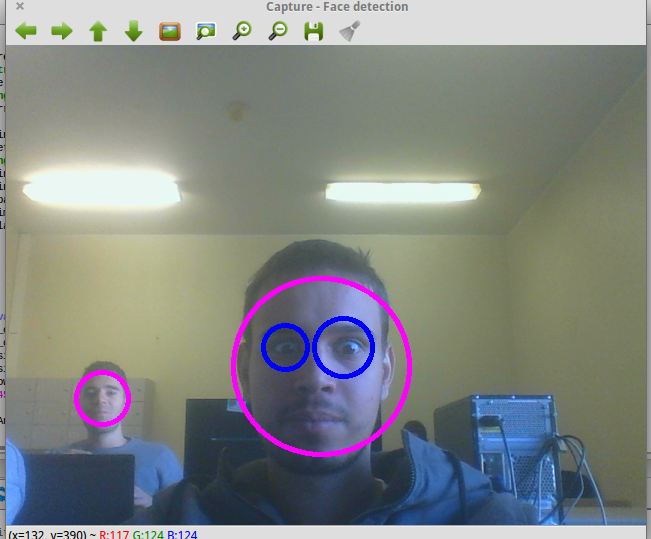
\includegraphics[width=70mm]{img/ex2_1.png}
\caption{Resultado obtido após exercício 2}
\end{figure}


%%%%%%%%%%%%%%%%%%%%%%%%%%%%%%%%%%%%%%%%%%%%%%%%%%%%%%%%%%%%%%5
%%%%%%%%%%%%%%%%%%%%%%%%%%%%%%%%%%%%%%%%%%%%%%%%%%%%%%%%%%%%%%%

\newpage
\subsection{Exercícios adicionais/opcionais}

Na questão do reconhecimento de sinais de trânsito pareceu-nos que o template matching não era o indicado para resolver o problema. Não só porque em imensos casos os algoritmos não encontravam o local certo na imagem a procurar, mas também porque esta implementação não ia funcionar em imensas circustâncias, como por exemplo, o ocultamento parcial do objeto a procurar.

Encontrámos um repositório com uma solução através da utilização de \textit{Gielis curves} e seguindo os passos de instalação do README que pode ser encontrado aqui \textit{https://github.com/glemaitre/traffic-sign-detection} conseguimos obter resultados surpreendentes. 

O resultado para a primeira imagem utilizada por nós no exercício 1 é o seguinte:

\begin{figure}[ht!]
\centering
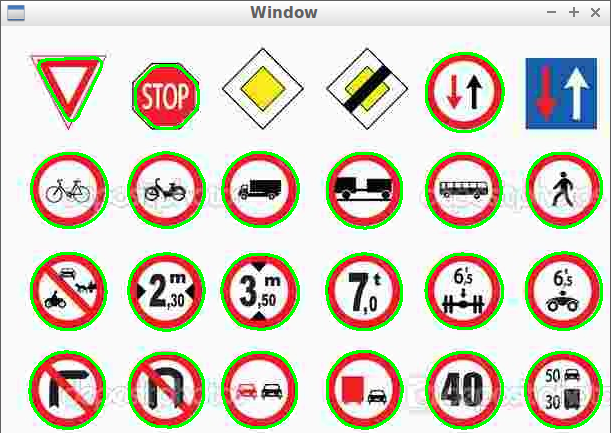
\includegraphics[width=70mm]{img/ex_adicional.png}
\caption{Resultado obtido após implementação adicional}
\end{figure}

O algoritmo usado aqui não usa template matching, mas é uma forma adicional muito interessante de resolver o exercício acima proposto. É primeiramente convertida a imagem rgb em ihls color space e em logarithmic chromatic vermelho e azul.

\begin{lstlisting}[caption=Image convertion,label=code:C]
 cv::Mat ihls_image;
colorconversion::convert_rgb_to_ihls(input_image, ihls_image);

std::vector< cv::Mat > log_image;
colorconversion::rgb_to_log_rb(input_image, log_image);
\end{lstlisting}

Depois é feito uma segmentação usando uma biblioteca específica \begin{lstlisting}[caption=Biblioteca usada,label=code:C]
#include <img_processing/segmentation.h>
segmentation::seg_norm_hue(ihls_image, nhs_image_seg_red, nhs_mode);
\end{lstlisting}

sendo a imagem processada similar a algo como:


\begin{figure}[ht!]
\centering
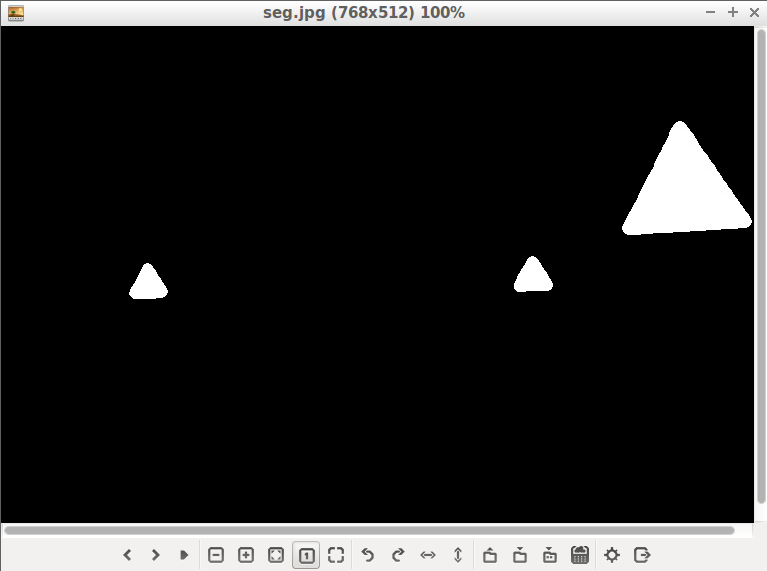
\includegraphics[width=70mm]{img/ex_adicional_seg.png}
\caption{Resultado obtido após segmentação}
\end{figure}

E é com essa imagem que depois fazem merge na original para se extrair os contornos.

\begin{lstlisting}[caption=Reconstrução do contorno,label=code:C]

std::cout << "Contour #" << contour_idx << ":\n" << final_config << std::endl;
std::vector< cv::Point2f > gielis_contour;
int nb_points = 1000;
optimisation::gielis_reconstruction(final_config, gielis_contour, nb_points);

...
        
std::vector< cv::Point > distorted_gielis_contour_int
    (distorted_gielis_contour.size());
for (unsigned int i = 0; 
    i < distorted_gielis_contour.size(); i++) {
    distorted_gielis_contour_int[i].x = (int) std::round(distorted_gielis_contour[i].x);
    distorted_gielis_contour_int[i].y = (int) std::round(distorted_gielis_contour[i].y);
}

\end{lstlisting}

Também é utlizado algoritmos para eliminar/corrigir a distorsão, normalizar o formato dos contornos, etc num código bem documentado. Este código pode ser encontrado na pasta traffic-sign-detection-master/src/main.cpp do nosso repositório dentro do diretório /aula10 e pode ser corrido da seguinte forma \textit{bin/main <path para a imagem>, ex: bin/main test-images/stop.jpg} que produzirá, por exemplo, os seguintes resultados:

\newpage

\begin{figure}[ht!]
\centering
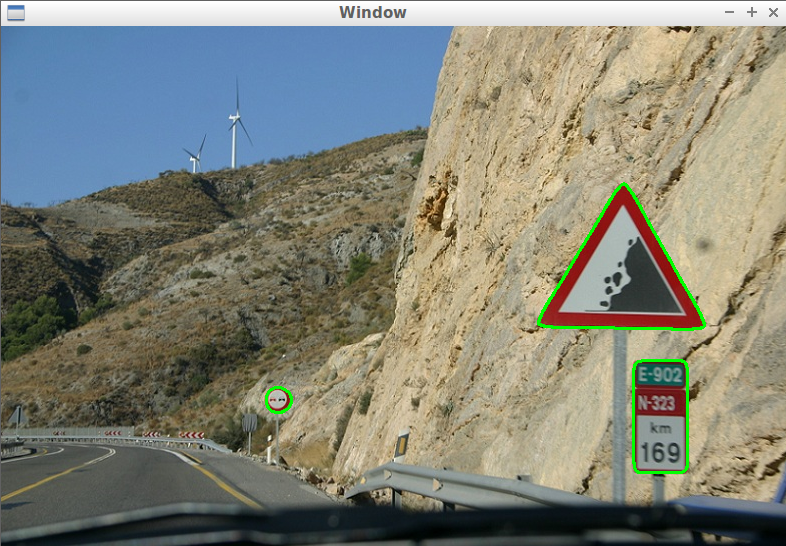
\includegraphics[width=70mm]{img/ex_adicional2.png}
\caption{Resultado obtido em imagem de contexto real}
\end{figure}

\begin{figure}[ht!]
\centering
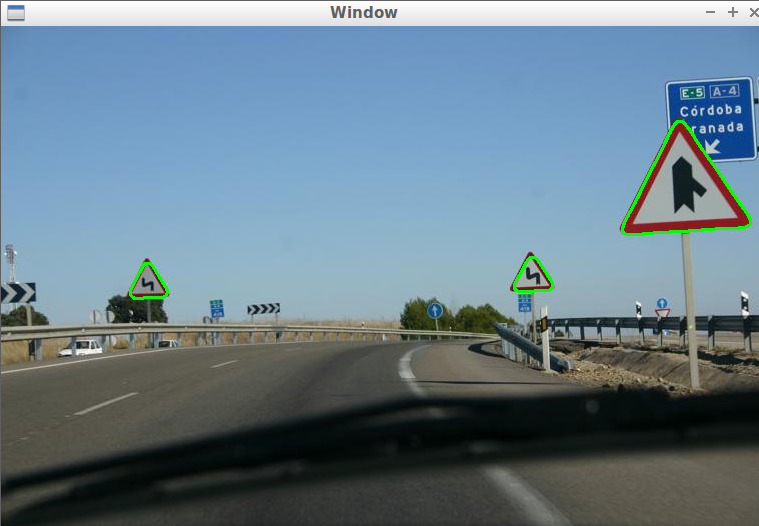
\includegraphics[width=70mm]{img/ex_adicional3.png}
\caption{Outro resultado em imagem num contexto real}
\end{figure}



%%%%%%%%%%%%%%%%%%%%%%%%%%%%%%%%%%%%%%%%%%%%%%%%%%%%%%%%%%%%%%5
%%%%%%%%%%%%%%%%%%%%%%%%%%%%%%%%%%%%%%%%%%%%%%%%%%%%%%%%%%%%%%%

\begin{thebibliography}{1} % 9

\bibitem{fsound}
Neves, A. J. R.; Dias, P. Slides teóricos Visão por Computador - Aula 10 (2016)

\bibitem{vtk}
OpenCV. \href{hhttp://docs.opencv.org/}{Opencv Documentation}. Web. 15 Outubro 2016. 

\bibitem{vtk}
Github. \href{https://github.com/glemaitre/traffic-sign-detection
}{traffic-sign-detection}. 8 Setember 2015.




\end{thebibliography}

\end{document}
